\documentclass{article}
\usepackage[utf8]{inputenc}
\usepackage[T2A]{fontenc}
\usepackage[utf8]{inputenc}
\usepackage{float}
\usepackage[russian]{babel}
\usepackage[a4paper, left=10mm, right=10mm, top=20mm, bottom=20mm]{geometry}
\usepackage{natbib}
\usepackage{graphicx}
\usepackage{tabularx}


\title{Описание FIT readout unit}
\author{Финогеев Дмитрий, ИЯИ РАН}





\begin{document}

\maketitle

Актуальная версия докумена доступна для скачивания по ссылке
\newline
https://github.com/dfinogee/FIT-readout-manual/archive/master.zip



\tableofcontents
\newpage

\section{FIT readout unit}
FIT readout unit (FRU) является модулем программного обеспечения ПЛИС плат PM/TCM. Основные функции FRU:

\begin{itemize}
\item Получение и обработка данных с CTP (через CRU): Триггеры, BC, Orbit 
\item Формирование пакета данных полученных с PM/TCM для каждого события (event packet, EP)
\item Отбор данных по триггеру в зависимости от режима набора данных
\item Формирование RDH пакета содержащего набор EP в соответствии требованиями ALICE DAQ 
\item Отправка RDH пакета в CRU по протоколу GBT
\end{itemize}


Функциональная схема FRU представлена на рис ~\ref{fig:2}
\begin{figure}[H]
	\centering 
	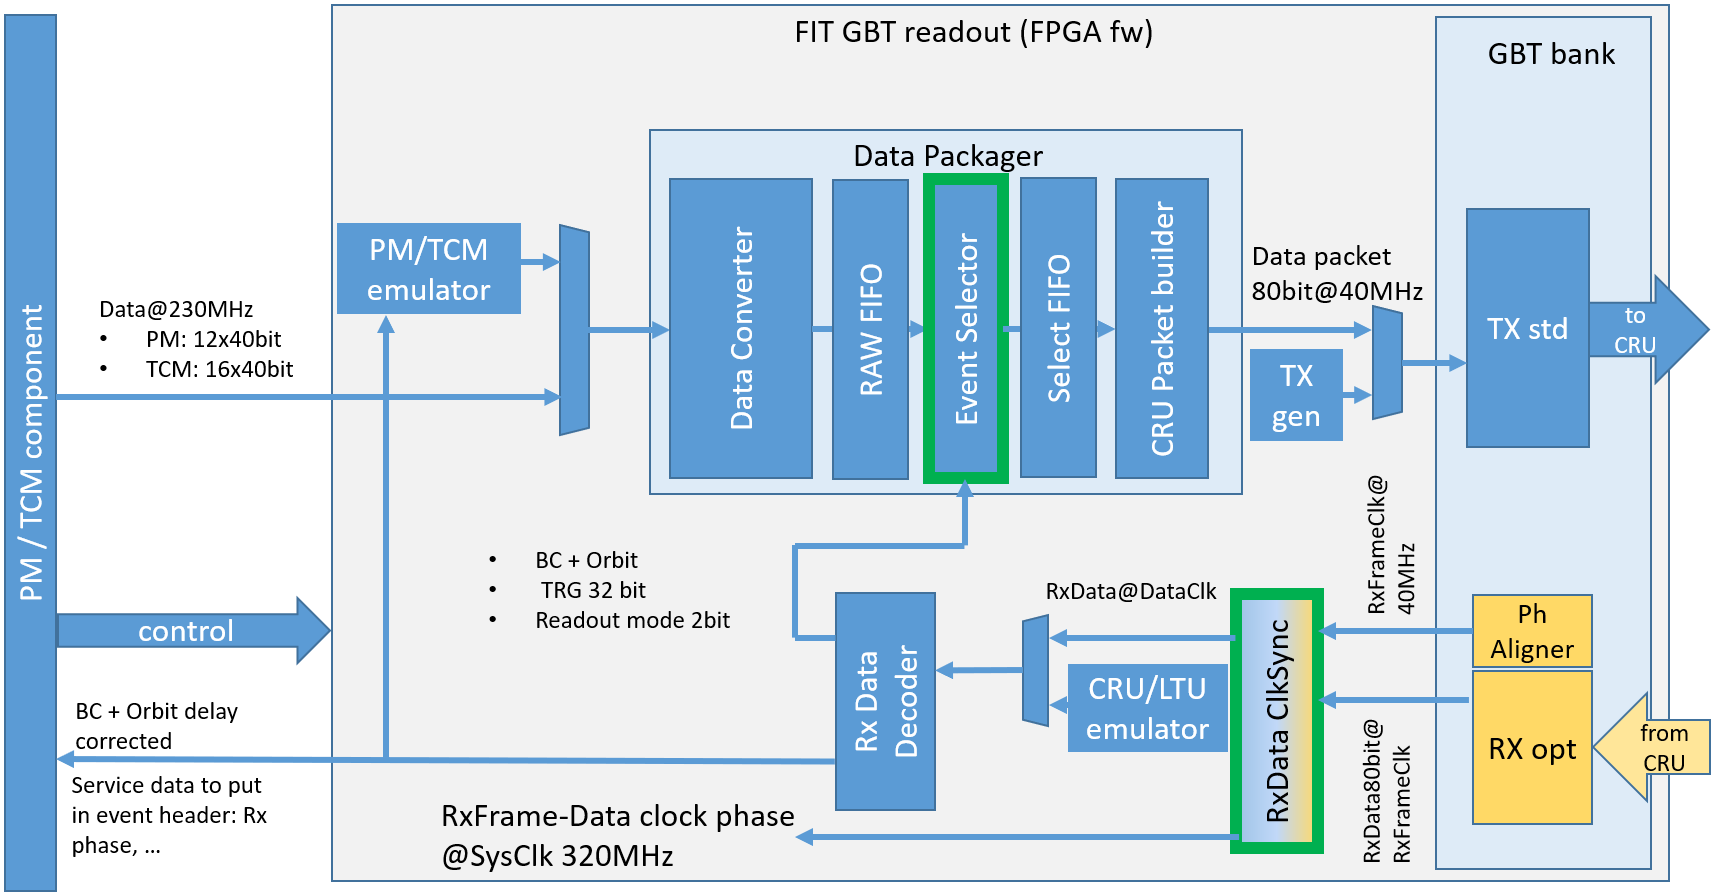
\includegraphics[width=1\textwidth]{FIT_readout.png}
	\caption{\label{fig:2} Функциональная схема FIT readout unit}
\end{figure}


FRU обменивается данными с PM/TCM с одной стороны и с CRU с другой. Данные в/из CRU передаются по оптической линии по протоколу GBT. Ширина шины составляют 80 бит и тактируются по клоку 40 МГц синхронным с CRU. Данные содержат информацию  orbit и bc 32 и 12 бит соответственно и триггерную информацию - 32 бита каждый из которых отвечает за соответствующие триггера включая триггера запуска и остановки рана, триггер физического события. Данные полученные по GBT передаются в модуль 'RxDataClkSync' для синхронизацией с внутренним клоком 40МГц, фаза между клоками измеряется по клоку 320МГц. После синхронизации данные передаются в модуль 'RX Data Decoder' где принимаются команды запуска и остановки рана и данные о BC и orbit. Данные BC и Orbit корректируются в соответствии с задержкой и отправляются в программный модуль PM/TCM. Для тестов без CRU предусмотрен модуль 'CRU/LTU emulator' в котором генерируются данные содержащие информацию  orbit и bc и триггерную информацию включая триггера запуска и остановки рана, триггер физического события.


Данные из PM/TCM передаются по клоку 320МГц и обрабатываются модулем 'Data Packager', для тестов на отладочной плате предусмотрен модуль 'PM/TCM emulator' позволяющий генерировать данные с PM/TCM. Модуль 'Data Packager' содержит подмодули 'Data Converter', 'Event selector' и 'CRU Packet builder'. Модуль 'Data Converter' формирует пакеты данных полученных с PM/TCM для каждого события (event packet, EP) и отправляет их в буфер памяти 'RAW FIFO' по клоку 320 МГц. Модуль 'Event Selector' принимает EP из памяти 'RAW FIFO' по клоку 320МГц, отбирает события в соответствии с триггером в триггерном режиме передачи и группирует данные в RDH пакеты в соответствии с требованиями ALICE DAQ. Отобранные и сгруппированные события с сопутствующей информацией необходимой для заголовка поступают в буфер памяти 'Select FIFO'. Третий модуль 'CRU Packet Builder' принимает данные из блока памяти 'Select FIFO', дополняет сформированные данные RDH заголовком и отправляет результат в модуль GBT для дальнейшей передачи в CRU. Для проверки работы GBT передатчика предусмотрен 'TX generator' передающий постоянный паттерн на вход GBT.

\section{Описание алгоритма коррекции BC и отбора событий}
На рис ~\ref{fig:3} представлена схема временной коррекции и алгоритма отбора событий. 

\begin{figure}[H]
	\centering 
	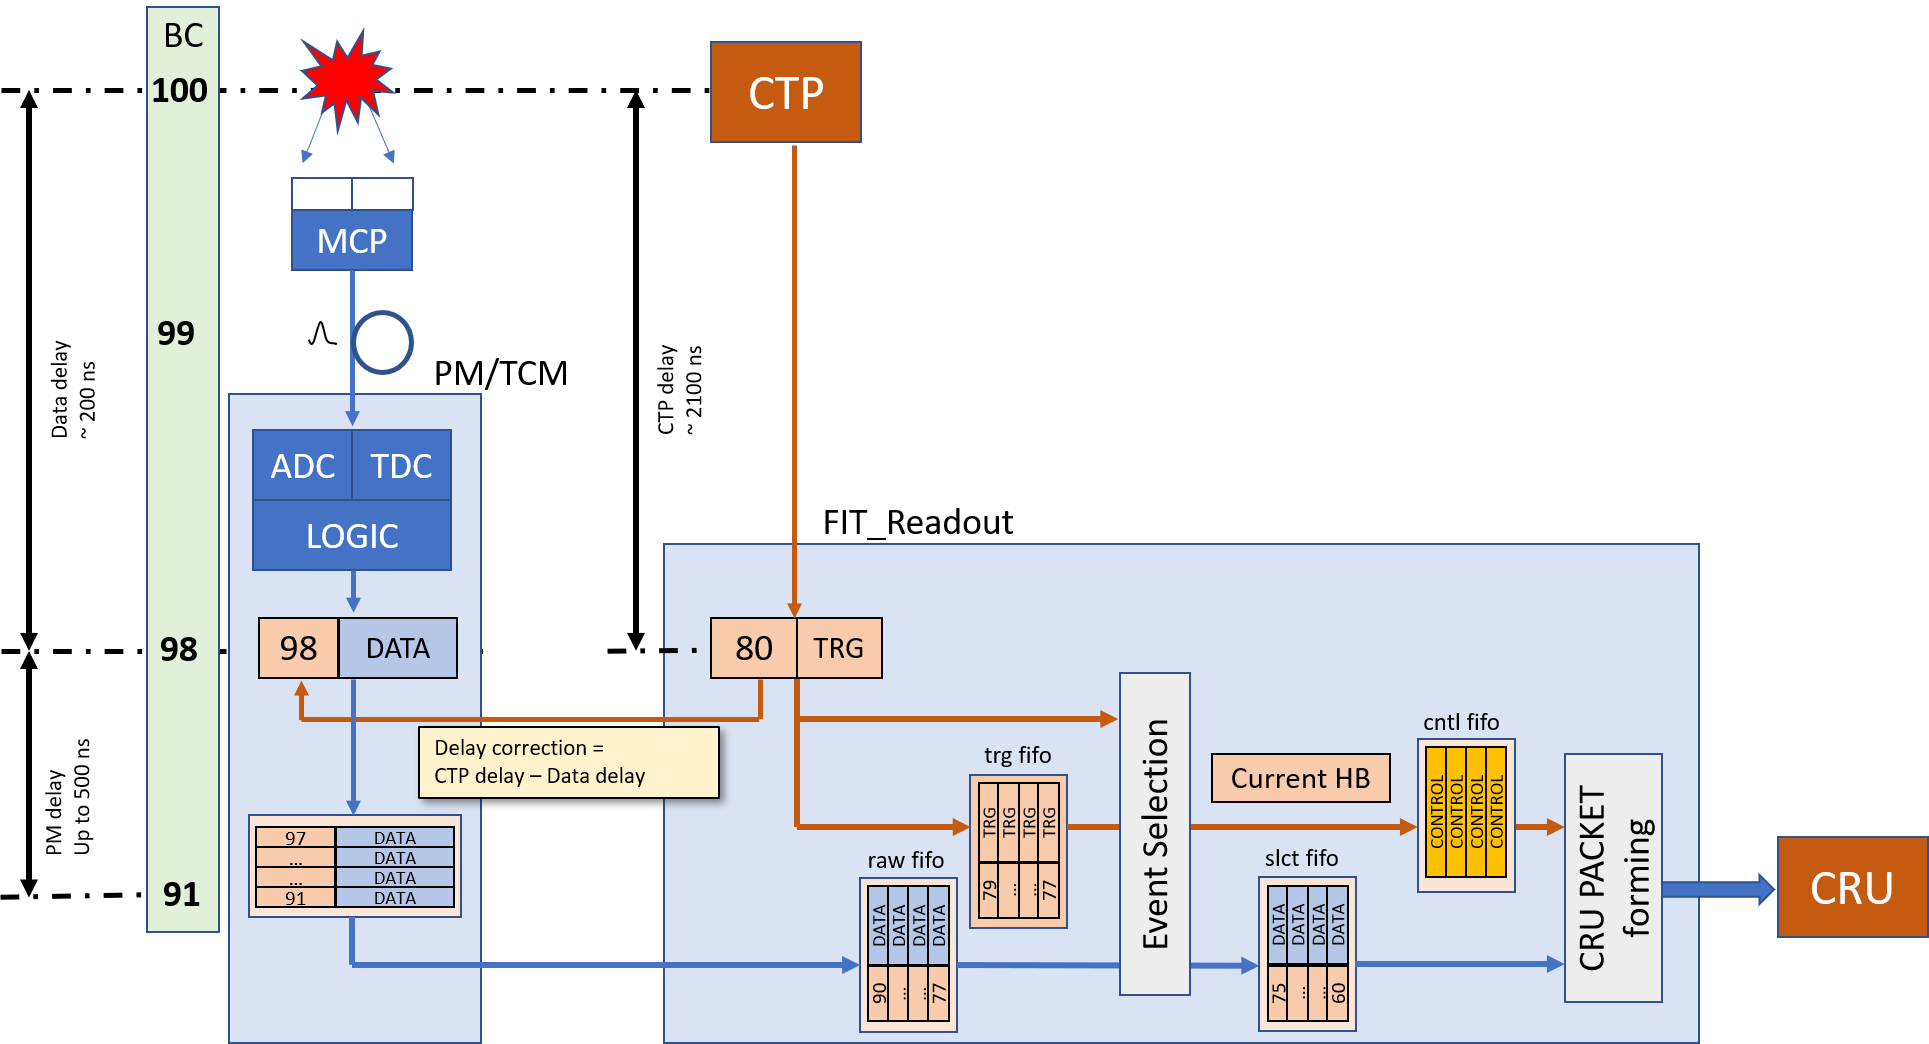
\includegraphics[width=1\textwidth]{BCIDcorr.png}
	\caption{\label{fig:3} Схема временной коррекции BC и отбора событий по триггеру}
\end{figure}

%Ускоритель LHC работает на частоте 40МГц что означает кратность времени между соударениями в 25нс. Отношение длинны накопительного кольца ускорителя к расстоянию между банчами частиц является целым постоянным числом равным 3564. Иными словами, кольцо ускорителя располагает 3564 слотами где могут находится банчи (группы) частиц. Эти банчи вращаются в двух кольцевых йонопроводах в противоположном направлении и сталкиваются между собой в четырех interaction points (IP): ATLAS, CMS, LHCb, ALICE. Между собой сталкиваются не каждые банчи, но время между столкновениями можно выразить количеством периодов клока 40МГц.

Каждое столкновение (событие, event) в ALICE@LHC пронумеровано двумя целыми числами: BC - порядковым номером банча в орбите (кольце ускорителя) 0 - 3563 (12 бит) и Orbit - порядковым номером орбита (32 бита).

Каждому событию в эксперименте ALICE соответствует триггерное решение, которое говорит о характере данного события. Так же существуют технические триггеры. Примеры триггеров: команды запуска и остановки набора данных в непрерывном и триггерном режимах (SOC, SOT, EOC, EOT), триггер отброса данных (HBr), триггер начала орбита (Orbit) и другие. Каждому триггеру соответствует один бит в 32 битном слове, каждому событию может соответствовать несколько триггеров. Номер и триггерное решение для каждого события посылается модулем Central Trigger Processor (CTP) с частотой 40МГц. Данная информация поступает в FIT Readout unit по протоколу GBT через модуль Common readout Unit (CRU) с задержкой порядка нескольких микросекунд.

На схеме рис ~\ref{fig:3} эти данные обозначены оранжевой стрелочкой от модуля CRU, для примера, на схеме текущий поступивший в FRU номер обозначен 16 и триггерное решение TRG для данного события. На схеме, для примера, происходит событие под номером 100. Регистрация и оцифровки события детектором происходит с задержкой, для примера на схеме задержка равна 8. Как задержка регистрации сигнала, так и задержка триггерного сигнала постоянны и известны. Задержка регистрации сигнала меньше чем задержка триггерного сигнала и для определения номера регистрируемого события, к номеру полученному от CTP прибавляется разница между задержками регистрации сигнала и распространение триггерного сигнала. На схеме эта разница равна (2100нс - 200нс)/25 = 76 и прибавив 76 к полученному номеру от CTP 16 получаем номер регистрируемого события 92. Данная операция выполняется в модуле 'RxDataDecoder', задержка определяется регистром 'BCID delay'. 

Триггерная информация, поступившая от CTP относится к поступившем вместе с ней номером события (на схеме 16-TRG). Она необходима для отбора и сортировки событий по триггеру и сохраняется в буфер памяти 'trg fifo'. Поскольку задержка регистрации событий меньше, чем задержка триггерного сигнала данные о событиях сохраняются в буфер памяти 'raw fifo' для дальнейшей сортировки. Сортировка на схеме обозначена блоком 'Event selection' и на входе принимает данные о текущем принятом номере события от CTP, и данные из буферов памяти 'raw fifo' и 'trg fifo' для сравнения.

Модуль 'Event Selection' выполняет сравнение номеров события для триггерного сообщения и данных детектора из 'raw data fifo' и 'trg fifo'.
\begin{itemize}
\item Если номер для триггерного сообщения меньше (соответствует более раннему событию) или данные в 'raw fifo' отсутствуют то это означает что данные для этого триггерного сообщения отсутствуют. В этом случае триггерное сообщение вычитывается из 'raw fifo' и при необходимости формируется RDH пакет (на пример при получении 'HB trigger').

\item Если номер события в данных меньше чем номер в триггерном сообщении то это означает что для данных отсутствует триггерное решение. В случае непрерывной передачи 'continuous readout' данные вычитываются из 'raw fifo' и передаются в 'select fifo' для формирования RDH. В случае триггерной передачи 'triggered readout' данные вычитываются из 'raw fifo' и отбрасываются в соответствии с алгоритмом отбора по триггеру.

\item Если номер события в данных равен номеру в триггерном сообщении то это означает что триггерное сообщение соответствует данным детектора. В случае непрерывной передачи 'continuous readout' данные вычитываются из 'raw fifo' и передаются в 'select fifo' для формирования RDH. В случае триггерной передачи 'triggered readout' данные вычитываются из 'raw fifo' и передаются в 'select fifo' для формирования RDH только при наличии необходимого триггера для отбора событий. Маска для отбора триггеров содержится в регистре 'Data select trigger mask'. Триггерное сообщение так же вычитывается из 'trg fifo'.

\item Если присутствуют данные детектора и отсутствует триггерное сообщение то это означает что триггерное сообщение может прийти позже. В этом случае выполняется сравнение номера события данных и текущего принятого номера события из CTP. Если разница между этими событиями больше фиксированной величины, то это означает что триггерное сообщение отсутствует для данных, данные вычитываются из буфера 'raw fifo' и отбираются в соответствии с режимом вычитывания данных. Если разница меньше или равна фиксированной величине, то данные сохраняются в 'raw fifo'. Величина для сравнения задается регистром 'Trigger compare delay'.
\end{itemize}

Для формирования RDH пакета данные отобранные из 'raw fifo' помещаются в 'selected fifo'. Для отправления RDH пакета при накоплении максимального объема данных или при иной необходимости (на данный момент согласно требованиям DAQ ALICE необходимо отправлять пакет при получении 'HB trigger' и для отправки 'HB stop frame') формируется управляющее слово. Управляющее слово содержит количество слов в RDH пакете и сопутствующую информацию для RDH заголовка в том числе номер орбита, триггерное решение (актуально для RDH v4). Модуль 'CRU Packet builder' принимает управляющее слово, вычитывает соответствующее количество слов из 'Selected fifo', формирует RDH пакет включая данные из регистров 'FEE ID', 'PAR', 'Detector field' (актуально для RDH v4) и отправляет его в модуль GBT.




\section{Описание функциональных модулей}
\subsection{модуль Event Selector}
Назначение модуля описано в разделе "Описание алгоритма коррекции BC и отбора событий". Модуль 'Event selector' принимает данные и триггерные сообщения для сравнения и отбора событий. Отобранные события помещаются в 'selected fifo' и сопровождаются командными словами для формирования RDH пакетов.

Каждое событие (40 МГц) модуль PM может сформировать до 6 слов плюс одно слово заголовки события, модуль TCM формирует одно слово плюс слово заголовка (в отладочном режиме 9+1 слов, допускается пропуск событий). Пакеты модуля передаются по клоку 320 МГц и максимальная длинна пакета для одного события (40 МГц) составляет 8 слов. Модуль 'Event selector' также читает и обрабатывает данные по клоку 320 МГц. 'selected fifo' читается модулем 'CRU packet builder' по клоку 40 МГц, GBT модуль так же передает данные по клоку 40 МГц. В связи с тем что 'selected fifo' читается по клоку 320 МГц а записывается по клоку 40 МГц, возможно его переполнение. В случае когда в 'selected fifo' не остается места для данных, данные отбрасываются. В этом случае запоминаются первый и последний номер орбита и количество пропущенных событий, эта информация доступна в регистрах 'first hit dropped orbit', 'last hit dropped orbit', 'selector hits dropped'. В регистре 'readout rate' отображается количество слов данных (80бит 40МГц) за последний орбит. В регистре 'selector fifo count' доступна занятость 'selector fifo'. Бит 'reset drop counter' в регистре 'Reset control' (при записи в него значения 0х1) позволяет сбросить счетчик пропущенных событий.

Регистр 'is HB response' (при значении 0х1) позволяет отключить отправку RDH пакета по получению триггера HB для снижения потока данных при использовании FTM.
Регистр 'Max RDH payload' задает максимальное количество слов в RDH пакете. Максимальный объем RDH пакета составляет 8 Кб, поскольку каждое переданное GBT слово дополняется в CRU до 128 бит, максимум в RDH пакете может содержаться 8192*8/128=512 слов GBT. Значение регистра означает количество GBT слов и должно быть равно 0х200. Для отладки максимальный размер пакета может быть уменьшен.
Регистр 'CRU trigger delay' определяет как долго данные модуля 'ожидают' триггерное сообщение (см. раздел "Описание алгоритма коррекции BC и отбора событий").
Регистр 'data select trigger mask' определяет маску (набор) триггеров для отбора в режиме триггерного вычитывания ('triggered mode').  При значении регистра 'readout mode' равном 'idle' модуль 'event selector' прекращает работу.



\subsection{модуль RX Data Decoder}
Модуль предназначен для обработки данных полученных от CRU (CTP) по GBT. Как описано в разделе "Описание алгоритма коррекции BC и отбора событий" каждому событию соответствует номер и триггерное решение. Допускается что триггерное сообщение, содержащее текущий номер события, может приходить не каждый клок 40 МГц, в случае если триггер отсутствует сообщение может быть пропущено (относится к первым требованиям ALICE DAQ). В связи с чем модуль 'RX data decoder' содержит внутренний счетчик событий, который может находится в трех состояниях 'Start', 'Sync', 'Lost', состояние счетчика доступно в регистре 'BCID sync mode'. При включении или по команде 'reset orbit sync' (бит 'reset orbit sync' в регистре 'reset control') счетчик переходит в состояние 'start' до получения первого триггера. После получения триггера счетчик переходит в состояние 'sync' и начинает отчет событий с полученного номера от CTP. Для определения номера события используется текущее значение счетчика в связи с чем получение каждого номера события от CTP не обязательно. Текущее значение номера события доступно из регистров 'CRU orbit', 'CRU bc'. При получении триггерного сообщения номер события полученный от CTP сравнивается со значением счетчика. Если эти значения не равны, то это означает рассинхронизацию внутреннего счетчика с нумерацией CTP, счетчик переходит в состояние 'lost' до момента получения сигнала 'reset orbit sync'.


Как было описано в разделе "Описание алгоритма коррекции BC и отбора событий" номер полученный от CTP, (фактически - номер внутреннего счетчика синхронизированный с CTP) корректируется на величину разности задержек в распространении триггерного сообщения и обработки сигнала детектором. Величина корректировки задается регистром 'bcid delay'.

Модуль 'RX data decoder' обрабатывает триггера запуска и остановки вычитывания (SOT - start of trigger, EOT - end of trigger, SOC - start of continuous, EOC - end of continuous) управляя текущем режимом вычитывания. Состояние режима может принимать значения 'idle', 'continuous', triggered', значение доступно по регистру статуса 'readout mode'. Выставив в регистре управления 'readout mode' бит 'force readout idle mode' возможно принудительно перевести режим вычитывания в 'idle' что необходимо при включении или возникновении ошибки. При значении регистра 'readout mode' равном 'idle' модуль 'event selector' прекращает работу.




\subsection{модуль CTP emulator}
Для работы без CTP/LTU предусмотрен модуль 'CTP emulator' который производит все необходимые данные для отладки работы 'FIT readout unit'. Включение модуля (отключение приема сигналов CTP) происходит переключением регистра 'Trigger generator' в состояние 'Continuous generator'. 'CTP emulator' выполняет следующие функции:
\begin{itemize}
\item Генерация триггера 'HB' и номера события event id для эмуляции CRU.
\item Генерфция триггеров запуска и остановки процедуры вычитывания.
\item Генерация одиночного триггера по команде
\item Генерация непрерывного триггера с возможностью синхронизацией с тестовым генератором данных
\end{itemize}
Генерация триггера 'HB' и номера события event id происходит автоматически и не управляется.

Генерация триггеров запуска и остановки процедуры вычитывания происходит по команде. При переводе регистра 'readout command' из состояния 'OFF' в состоянии команды 'SOC', 'SOT', 'EOT', 'EOC' отправляется соответствующий триггер управления режимом вычитывания. Триггер команды отправляется в момент начала орбита вместе с триггером 'HB' в соответствии с требованиями ALICE DAQ.

Для отправки единичного триггера необходимо в регистр 'trigger single value' записать ноль, а потом значение триггера, которое необходимо отправить. Отправка триггера происходит при изменении регистра из значения 0x0 в ненулевое.



Генерация непрерывных триггеров по функциональности схожа с тестовым генератором данных модуля 'PM/TCM emulator'. Значение генерируемого триггера задается регистром 'continuous trigger value'. Регистрами 'trigger continuous pattern' формируется последовательность из 64 значений задающая очередность генерации триггера 'pattern'. Частота запуска 'pattern' определяется регистром 'trigger bunch frequency' задающим число отсчетов 'event id' между 'pattern'. Первая генерация 'pattern' происходит с отступом от начала орбита ('HB' trigger) на величину регистра 'trigger frequency offset' задающим число отсчетов 'event id'. Если частота 'pattern' равна велечине орбита (регистр 'trigger bunch frequency' равен 0xDEC) то сдвиг паттерна относительно 'HB trigger' будет постоянен. 

На рисунке ~\ref{fig:3} представлена схема генерации последовательности триггеров модулем 'CTP emulator'.

\begin{figure}[H]
	\centering 
	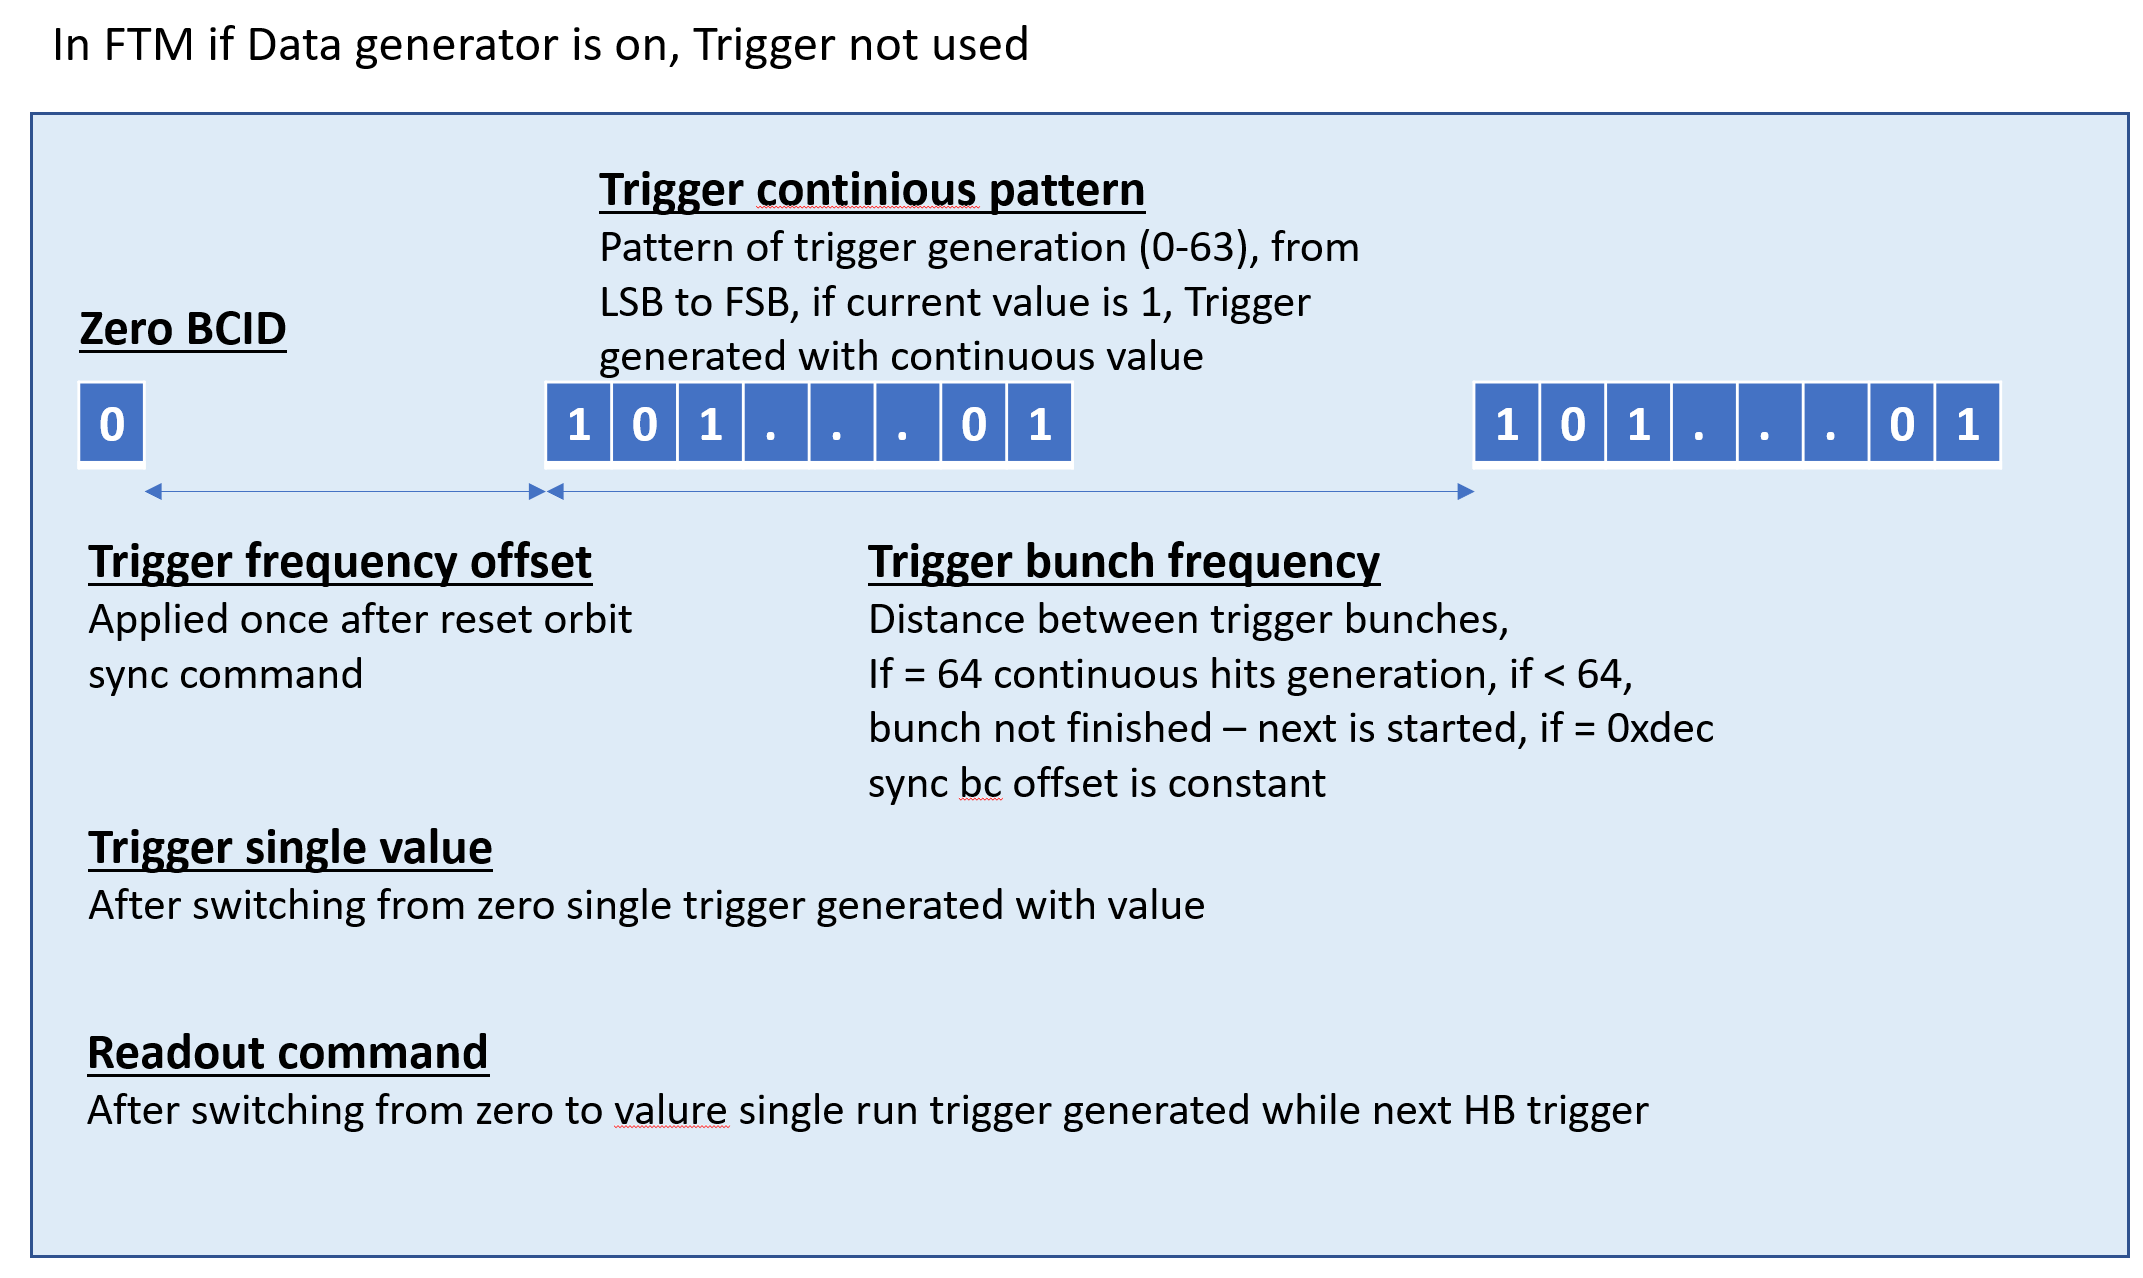
\includegraphics[width=0.8\textwidth]{trigger generator.png}
	\caption{\label{fig:4} Схема генерации последовательности триггеров модулем 'CTP emulator'}
\end{figure}



Так, на пример, если регистр 'trigger bunch frequency' равен 0xDED, регистр 'trigger frequency offset' равен 0x5 то в момент старта генератора или при переходе бита 'reset start offset' в регистре 'reset control' из состояния 0х1 в 0х0 будет ожидаться следующий триггер 'HB'. При получении триггера 'HB' будет произведен отсчет в 0x5 событий 'event id'. После этого будет запущена генерация триггеров в соответствии с 'pattern'. Если регистр 'Trigger continuous pattern 31 to 0' равен 0x3 и 'Trigger continuous pattern 63 to 32' равен 0x1 то будет сгенерированы триггера на пятом, шестом и 38 событии в орбите. После этого будет произведен отсчет в 0хDED событий 'event id' и новый запуск генерации триггеров в соответствии с 'pattern'. Поскольку значение 0xDED на одно больше, чем длительность орбита, в следующем орбите триггера будут в событиях с номерами 6, 7 и 39.

Модуль 'PM/TCM emulator' имеет схожий алгоритм генерации что позволяет обеспечить генерацию данных синхронно с генерацией триггера для отладки работы механизма отбора событий.




\subsection{модуль Data converter}
Модуль 'data converter' принимает данные от PM/TCM по клоку 320 МГц и дополняет их заголовком 'event header'. Данные, дополненные заголовком оправляются в 'raw fifo' по клоку 320 МГц. Для контроля занятости 'raw fifo' по регистру 'raw fifo count' доступно количество слов данных в fifo.



\subsection{модуль TX data gen}
Для отладки GBT передачи возможно подать фиксированный пакет данных в передачи GBT переключив регистр 'Data generator' в режим 'TX generator'. Так же возможно выключить всю логику 'FIT readout unit' выставив в регистре 'Readout mode' бит 'is readout bypass mode'. В этом случае данные, полученные с модуля PM/TCM будут записываться во внутренне fifo по клоку 320 МГц и сразу же, без обработки, передаваться в GBT модуль по клоку 40 МГц.


\subsection{модуль GBT}
Описание работы модуля GBT доступно по ссылке https://espace.cern.ch/GBT-Project/GBT-FPGA. Статус модуля доступен в регистре 'gbt status'. При возникновении ошибки 'GBT RX error detected' бит 'GBT RX error latch' принимает состояние 0х1 до подачи сигнала 'reset GBT errors' (регистр 'Reset control'). Перезагрузка GBT модуля выполняется командой 'GBT reset' (регистр 'Reset control').


\subsection{модуль RX data clock sync}
На схеме ~\ref{fig:5} представлена схема регистров (логических защелок) для перехода между асинхронными клоками: внутренним клоком 'Data clk' 40 МГц и клоком от CRU 'RX frame clk' 40 МГц полученным через модуль GBT. Фаза между этими клоками измеряется по клоку 'system clk' 320 МГц и может принимать значения от 0 до 7. При нормальном режиме работы фаза не должна меняется больше чем на +-1 отсчета от значения при начале синхронизации, если это происходит значение бита 'RX phase error' регистра 'GBT status' принимает значение 0х1 до сброса командой 'reset RX phase error' регистра 'Reset control'




\begin{figure}[H]
	\centering 
	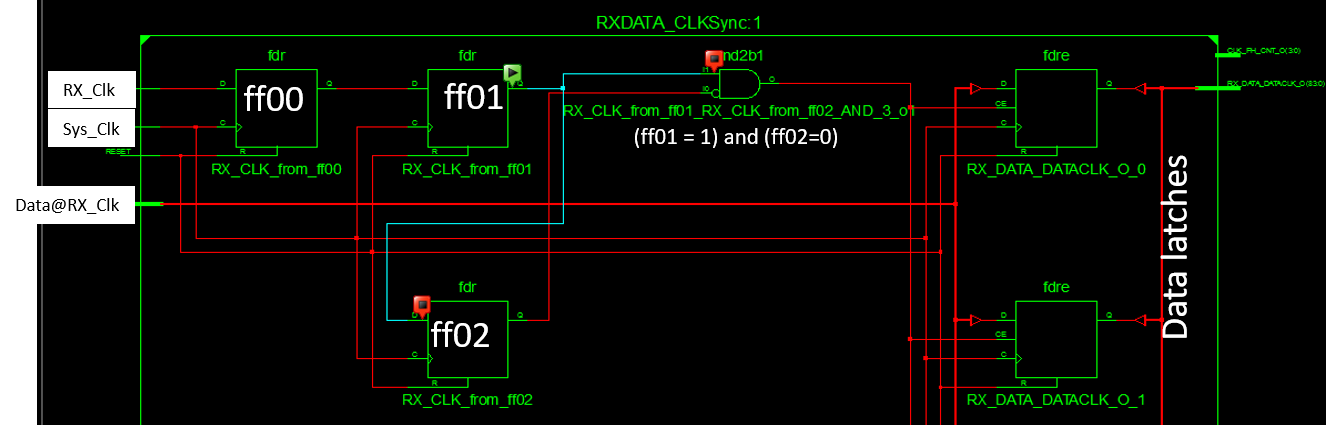
\includegraphics[width=1\textwidth]{cross_clock_domain_latch.png}
	\caption{\label{fig:5} Схема перехода между асинхронными клоками от RXframeClk 40Мгц от CRU и внутренним клоком Data clk 40 МГц}
\end{figure}



\subsection{модуль CRU packet builder}
Модуль 'CRU packet builder' принимает данные, сформированные модулем 'event selector' (см разделы "Описание алгоритма коррекции BC и отбора событий" и "модуль Event Selector") и формирует RDH пакет используя регистры 'FEE ID', 'PAR', 'DET field'.




\subsection{модуль PM/TCM emulator}
Данный модуль предназначен для отладки 'FIT readout unit' и генерирует данные от модуля PM/TCM, где в качестве значения данных, используется непрерывный счетчик. Для включения модуля в регистр 'Data generator' следует записать значение 'main generator'. Регистрами 'Data bunch pattern', 'data bunch frequency', 'data start offset' можно задавать последовательность, частоту, и смещение относительно орбита. Алгоритм генерации данных модуля схожа с генерацией непрерывного триггера в модуле модуле 'CTP emulator'. Отличие состоит в том, что при генерации тригерра 'pattern' состоит из 64 однобитных значений определяющих наличие триггера на данном шаге. В модуле 'PM/TCM emulator' 'pattern' задается восемью значениями по 4 бита (0-15). Каждое значение определяет количество слов в пакете для текущего события. В случае если значение превышает 0х6, то следующие события не генерируются пока не закончится передача текущего слова. Так на пример если значение регистра 'Data bunch pattern' равно 0х111D21 то последовательность пакетов будет следующая: пакет с одним словом, с двумя, с 13 (на шагах 4 и 5 пакеты генерироваться не будут), с одним словом.

Регистр 'trigger response mask' позволяет определить набор триггеров, при получении которых будет вырабатываться данные генератора с количество слов для первой позиции паттерна (если выполняется непрерывная генерация данных, то количество слов будет соответсвовать нулевой позиции 'pattern' а не текущему шагу). Следует отметить что номер события 'event id' пакета будет больше чем у триггера из-за задержки алгоритма. 

Бит 'reset start offset' в регистре 'Reset control' перезапускает генерацию данных в модулях 'PM/TCM emulator' и 'CTP emulator' для их синхронизации.




\section{Список ошибок и процедура их обработки}
При рассинхронизации номера события (регистр BCID sync mode перешел в состояние 'lost' или 'start') отправка событий в модуле 'event selector' останавливается.
Требуется процедура перезапуска вычитывания (еще не реализована)




\section{Описание клоков}
FIT readout unit использует две группы клоков с   произвольным  фазовым сдвигом: группа платы содержит два синхронных клока 'Data clk' 40 МГц и 'system clk' 320МГц, эти клоки  формируются на плате PM/TCM. Клок 40 МГц используется для работы с данными GBT, клок 320 МГц используется для обработки данных. 

Вторая группа клоков содержит клок 'RxFrameClk' 40МГц полученный из модуля GBT, синхронный CRU и используемый для передачи данных принятых данных с CRU. Данные принятые из CRU по клоку 'RxFrameClk' синхронизируются с группой клоков платы в модуле 'RxData ClkSync', в последующем клок 'RxFrameClk' не используется.

Физически клоки обеих асинхронных групп имеют один источник что обеспечивает одинаковую частоту.


\section{Описание формата данных детектора FIT}
Структура пакета передаваемых детектором по GBT приведена на рисунке  ~\ref{fig:6}. Заголовком пакета является  RDH (Raw Data Header) Актуальную версию формата заголовка можно узнать из комментариев к коду O2.

https://github.com/AliceO2Group/AliceO2/blob/dev/DataFormats/Headers/include/Headers/RAWDataHeader.h


\begin{figure}[H]
	\centering 
	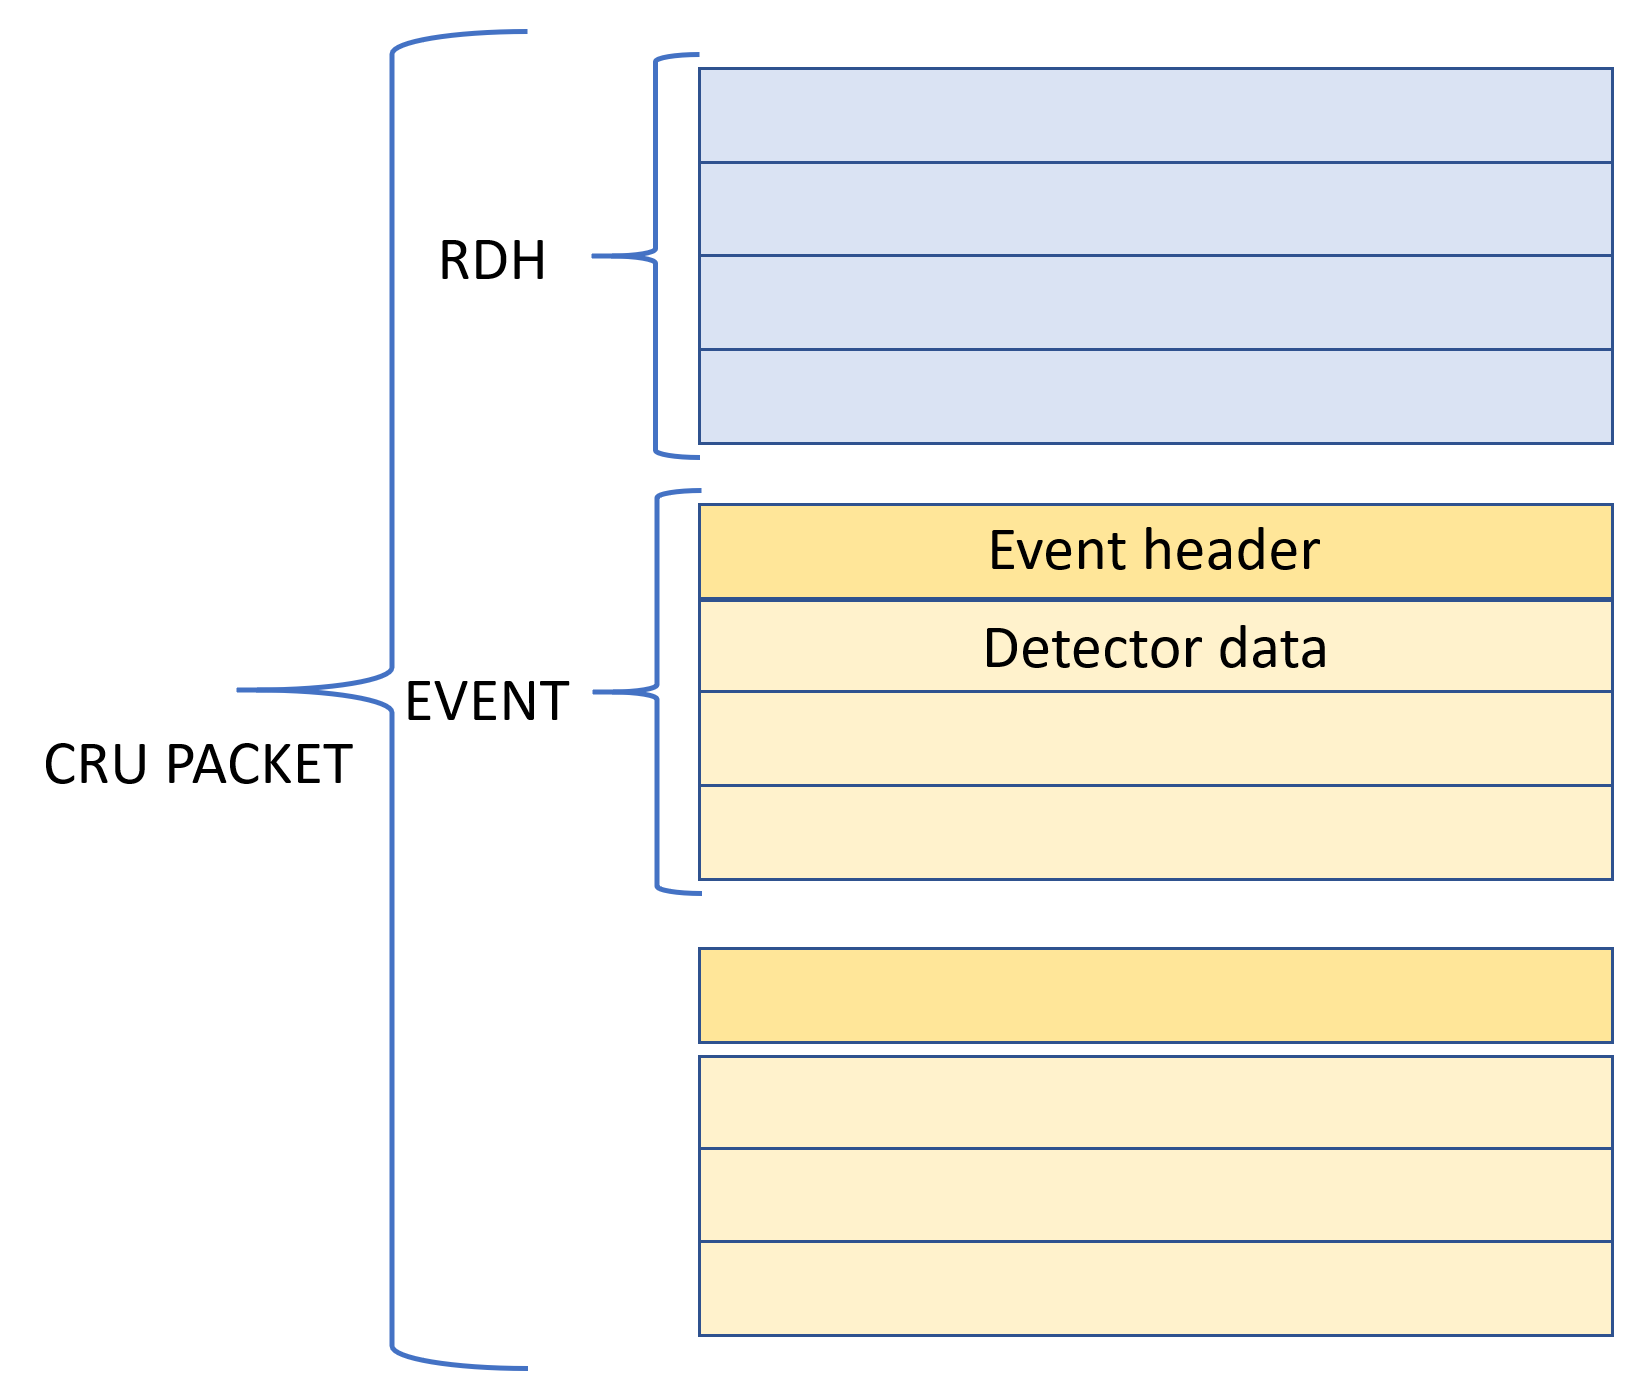
\includegraphics[width=0.5\textwidth]{RDH_scheme.png}
	\caption{\label{fig:6} Схема RDH пакета}
\end{figure}



В теле RDH пакета содержится набор пакетов данных каждый из которых относится к отдельному событию и состоит из заголовка 'event header' и блока данных. Пакеты событий всегда относятся к одному орбиту и отсортированы по порядку поступления. Формат заголовка одинаков для модулей PM/TCM, его формат представлен в таблице ~\ref{fig:7}. Формат блока данных различен для PM/TCM, TCM имеет два режима передачи: стандартный и расширенный. В PM каждое GBT слово 80 бит содержит одно или два слова 40 бит для канала: с 0 бита по 39 и с 40 по 79, в случае одного слова, старшие биты с 40 по 79 заполняются нулями. Формат слова для канала представлен в таблице ~\ref{fig:8}. Поскольку PM имеет 12 каналов, размер пакета данных события составляет от двух до 7 слов GBT. Формат данных для TCM представлен в таблице ~\ref{fig:9} и имеет размер в 1 GBT слово плюс заголовок. В расширенном режиме пакет данных TCM имеет 9 слов плюс заголовок в этом режиме передача данных для двух соседних событий невозможна. Актуальная версия формата данных доступна по ссылке.

https://drive.google.com/file/d/1LxKEuedLqxtyCRw072ZqJ2vj7upP0ZgV



\begin{figure}[H]
	\centering 
	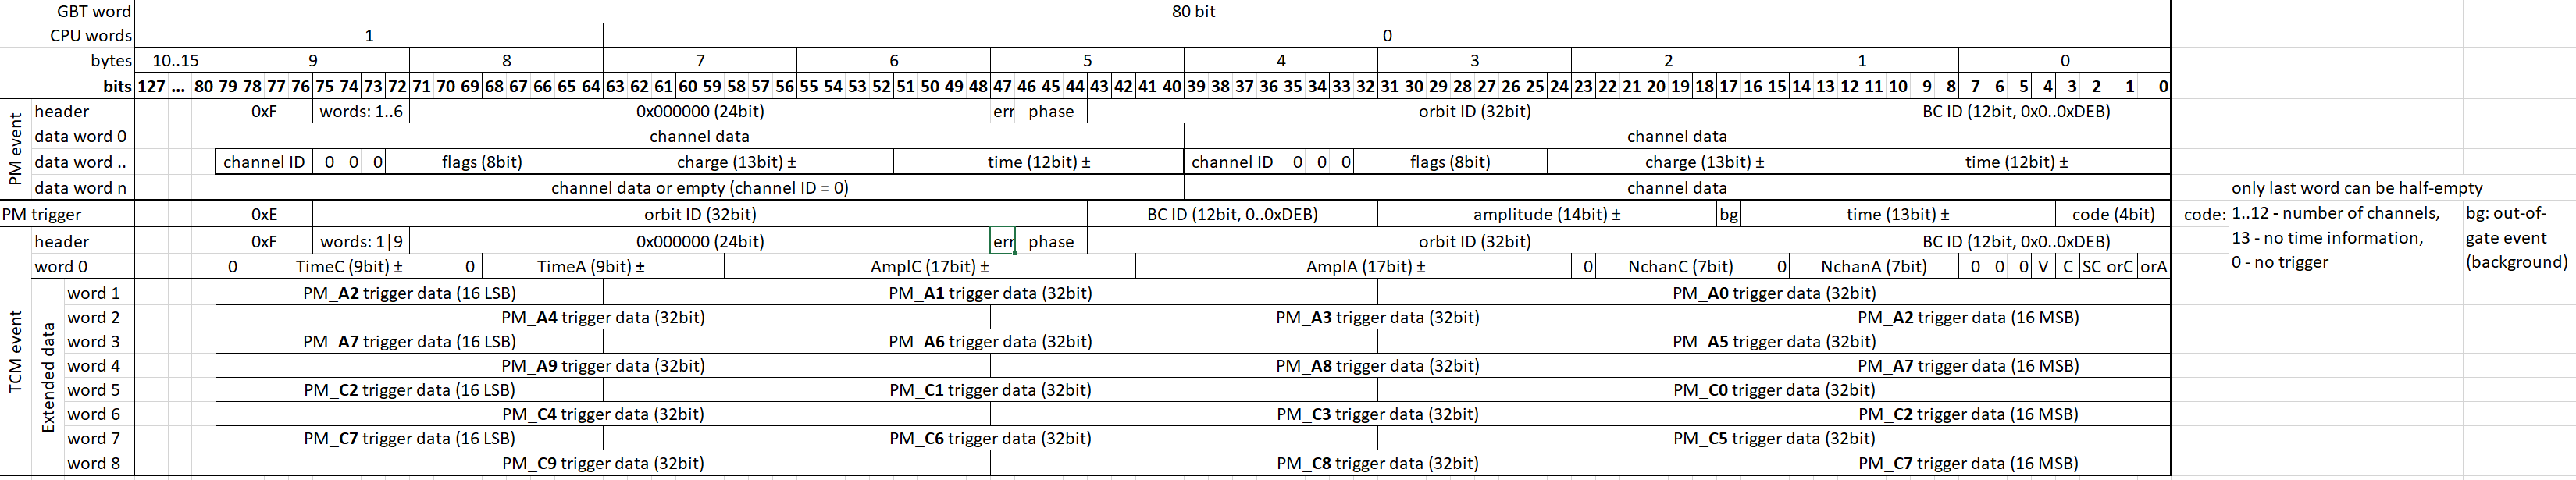
\includegraphics[width=1\textwidth]{readout_format.png}
	\caption{\label{fig:7} Формат данных детектора}
\end{figure}

\begin{figure}[H]
	\centering 
	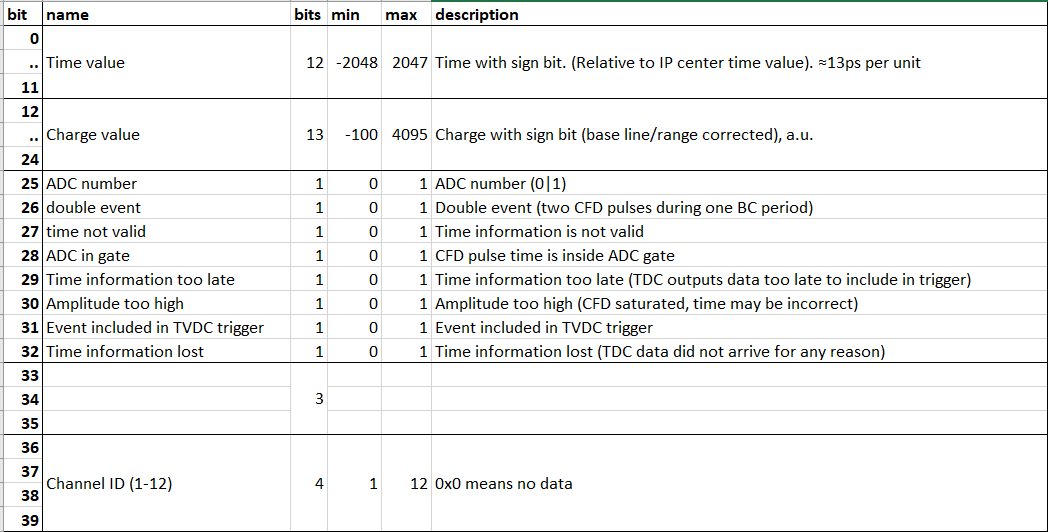
\includegraphics[width=0.8\textwidth]{PM_data.png}
	\caption{\label{fig:8} Формат данных модуля PM}
\end{figure}

\begin{figure}[H]
	\centering 
	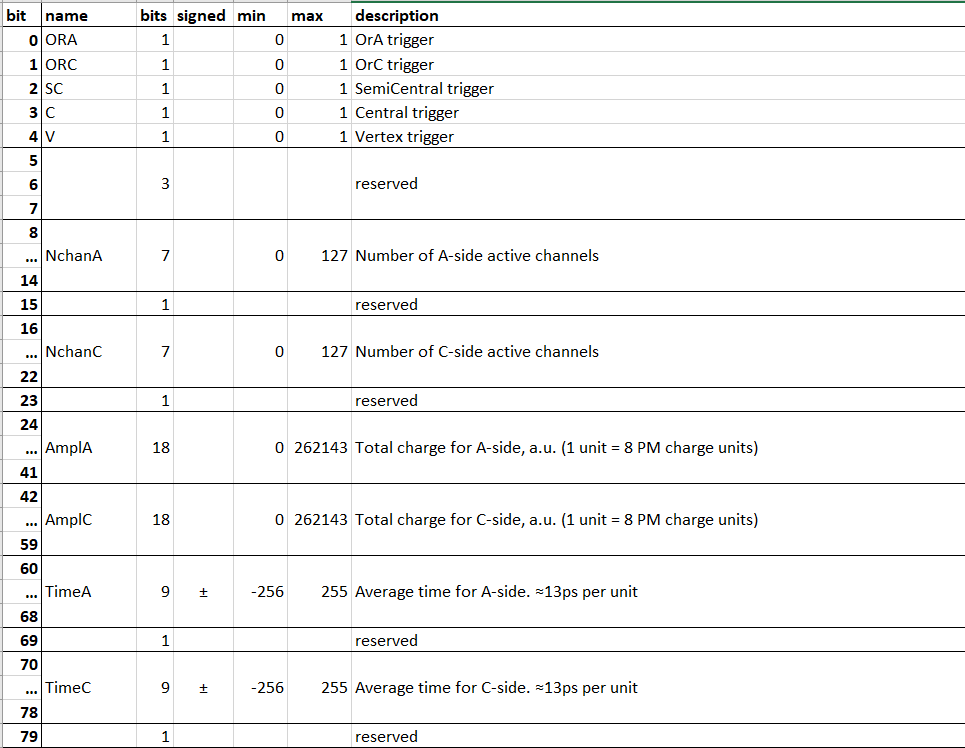
\includegraphics[width=0.8\textwidth]{TCM_data.png}
	\caption{\label{fig:9} Формат данных модуля TCM}
\end{figure}




\section{Используемые компоненты блоков памяти}


\begin{table}[H]
\begin{tabularx}{1\textwidth}{|p{1,8cm}|p{1cm}|p{1cm}|p{1cm}|p{1,5cm}|p{1,5cm}|p{1,5cm}|p{1,5cm}|X|}
\hline
Название & ширина записи, бит & ширина чтения, бит & размер & клок записи & клок чтения & используется в модуле & регистр занятости & назначение \\ \hline

Raw fifo & 80 & 80 & 4096 & system320 & system320 & Data packager & Raw FIFO count & Принимает сформированные данные PM/TCM для дальнейшего отбора модулем'event selector' \\ \hline

Selector fifo & 80 & 80 & 4096 & system320 & data40 & Data packager & Selector FIFO count & Принимает отобранные данные для формирования RDH \\ \hline

Trg fifo & 76 & 76 & 512 & data40 & system320 & event selector & нет & Принимает триггеры для отбора событий \\ \hline

Сntpck fifo & 160 & 160 & 128 & system320 & data40 & event selector & нет & содержит управляющие слова для формирования RDH \\ \hline

data320to40 & 80 & 80 & 4096 & system320 & data40 & TX data generator & нет & принимает данные модуля из raw data fifo для отправки по GBT в режиме 'is readout bypass mode' \\ \hline

\end{tabularx}
\caption{Список используемых блоков памяти\label{tab0}}
\end{table}





\section{Регистры управления и статуса}

\subsection{Описание регистров управления}


\begin{table}[H]
\centering
\begin{tabular}{| l | l | l |}
\hline
Название регистра & используется в модуле & является побитовым \\ \hline
Readout mode & Event selector, TX generator, RX data decoder & да \\ \hline
Readout command & CTP/LTU emulator & нет \\ \hline
Reset control & GBT, RX data decoder, Event selector, RX data clock sync & да \\ \hline
Trigger generator & CTP/LTU emulator & нет \\ \hline
Data generator & PM/TCM emulator & нет \\ \hline
Trigger response mask & CTP/LTU emulator & нет \\ \hline
Data bunch pattern & PM/TCM emulator & нет \\ \hline
Trigger single value & CTP/LTU emulator & нет \\ \hline
Trigger continuous pattern & CTP/LTU emulator & нет \\ \hline
Trigger continuous value & CTP/LTU emulator & нет \\ \hline
Trigger bunch frequency & CTP/LTU emulator & нет \\ \hline
Data bunch frequency & PM/TCM emulator & нет \\ \hline
Trigger start offset & CTP/LTU emulator & нет \\ \hline
Data start offset & PM/TCM emulator & нет \\ \hline
FEE ID & CRU packet builder & нет \\ \hline
PAR & CRU packet builder & нет \\ \hline
Max RDH payload &  Event selector & нет \\ \hline
Detector field & CRU packet builder & нет \\ \hline
Trigger compare delay &  Event selector & нет \\ \hline
BCID delay & RX data decoder & нет \\ \hline
Data select trigger mask &  Event selector & нет \\ \hline
%reg & module & да \\ \hline
\end{tabular}
\caption{Список регистров управления\label{tab1}}
\end{table}


\begin{table}[H]
\centering
\begin{tabular}{| l | l | l | l | l | l | l | l | l |}
\hline
addr & 31 .. 28 & 27 .. 24 & 23 .. 20 & 19 .. 16 & 15 .. 12 & 11 .. 8 & 7 .. 4 & 3 .. 0 \\ \hline
D8 &  &  & Readout mode & Readout command & \multicolumn{2}{c|}{Reset control} & Trigger generator & Data generator \\ \hline
D9 &  \multicolumn{8}{c|}{Trigger respond mask} \\\hline
DA &  \multicolumn{8}{c|}{Data bunch pattern} \\\hline
DB &  \multicolumn{8}{c|}{Trigger single value} \\\hline
DC &  \multicolumn{8}{c|}{Trigger continuous pattern 63 to 32} \\\hline
DD &  \multicolumn{8}{c|}{Trigger continuous pattern 31 to 0} \\\hline
DE &  \multicolumn{8}{c|}{Trigger continuous value} \\ \hline
DF &  \multicolumn{4}{c|}{Trigger bunch frequency} & \multicolumn{4}{c|}{Data bunch frequency} \\ \hline
E0 & & \multicolumn{3}{c|}{Trigger start offset} &  & \multicolumn{3}{c|}{Data start offset} \\ \hline
E1 &  \multicolumn{4}{c|}{FEE ID (RDH)} & \multicolumn{4}{c|}{PAR (RDH)} \\ \hline
E2 &  \multicolumn{4}{c|}{Max RDH payload} & \multicolumn{4}{c|}{Detector field (RDH)} \\ \hline
E3 &  \multicolumn{4}{c|}{Trigger compare delay} & \multicolumn{4}{c|}{BCID delay} \\ \hline
E4 &  \multicolumn{8}{c|}{Data select trigger mask} \\ \hline
\end{tabular}
\caption{Таблица адресов регистров управления.\label{tab2}}
\end{table}



\begin{table}[H]
\centering
\begin{tabular}{| l | l | l |}
\hline
No & bit & значение \\ \hline
0 & 8 & Orbit sync \\ \hline
1 & 9 & Drop hit counter \\ \hline
2 & 10 & Generator start offset \\ \hline
3 & 11 & GBT errors \\ \hline
4 & 12 & Reset GBT \\ \hline
5 & 13 & RX phase error \\ \hline
\end{tabular}
\caption{Описание битов регистра 'Reset control'\label{tab3}}
\end{table}



\begin{table}[H]
\centering
\begin{tabular}{| l | l | l |}
\hline
Значение регистра & режим работы \\ \hline
0 & No generator \\ \hline
1 & Main generator \\ \hline
2 & TX generator \\ \hline
\end{tabular}
\caption{Описание состояний регистра 'Data generator'\label{tab4}}
\end{table}


\begin{table}[H]
\centering
\begin{tabular}{| l | l | l |}
\hline
Значение регистра & режим работы \\ \hline
0 & No generator \\ \hline
1 & Continuous generator \\ \hline
\end{tabular}
\caption{Описание состояний регистра 'Trigger generator'\label{tab5}}
\end{table}


\begin{table}[H]
\centering
\begin{tabular}{| l | l | l |}
\hline
Значение регистра & режим работы \\ \hline
0 & None \\ \hline
1 & SOC \\ \hline
2 & SOT \\ \hline
3 & EOC \\ \hline
4 & EOT \\ \hline
\end{tabular}
\caption{Описание состояний регистра 'Readout command'\label{tab6}}
\end{table}


\begin{table}[H]
\centering
\begin{tabular}{| l | l | l |}
\hline
No & bit & значение \\ \hline
0 & 20 & Is HB response \\ \hline
1 & 21 & Is readout bypass mode \\ \hline
2 & 22 & Force readout idle mode \\ \hline
\end{tabular}
\caption{Описание битов регистра 'Readout mode'\label{tab7}}
\end{table}


\subsection{Описание регистров статуса}

\begin{table}[H]
\centering
\begin{tabular}{| l | l | l |}
\hline
Название регисра & используется в модуле & является побитовым \\ \hline
RX phase & RX data clock sync & нет \\ \hline
BCID sync mode & RX data decoder & нет \\ \hline
Readout mode & RX data decoder & нет \\ \hline
GBT status & GBT, RX data clock sync & да \\ \hline
CRU orbit & RX data decoder & нет \\ \hline
CRU bc & RX data decoder & нет \\ \hline
Selector FIFO count & Event selector & нет \\ \hline
Raw FIFO count & Data converter & нет \\ \hline
Selector first hit dropped orbit & Event selector & нет \\ \hline
Selector last hit dropped orbit & Event selector & нет \\ \hline
Selector total hits dropped & Event selector & нет \\ \hline
Readout rate & Event selector & нет \\ \hline
\end{tabular}
\caption{Список регистров статуса\label{tab8}}
\end{table}


\begin{table}[H]
\centering
\begin{tabular}{| l | l | l | l | l | l | l | l | l |}
\hline
addr & 31 .. 28 & 27 .. 24 & 23 .. 20 & 19 .. 16 & 15 .. 12 & 11 .. 8 & 7 .. 4 & 3 .. 0 \\ \hline
E8 &  & RX phase & BCID sync mode & Readout mode & \multicolumn{4}{c|}{GBT status}\\ \hline
E9 &  \multicolumn{8}{c|}{CRU Orbit} \\\hline
EA &  & & & & & \multicolumn{3}{c|}{CRU BC} \\\hline
EB &  \multicolumn{4}{c|}{Selector FIFO count} &  \multicolumn{4}{c|}{Raw FIFO count} \\\hline
EC &  \multicolumn{8}{c|}{Selector first hit dropped orbit} \\\hline
ED &  \multicolumn{8}{c|}{Selector last hit dropped orbit} \\\hline
EE &  \multicolumn{8}{c|}{Selector total hits dropped} \\ \hline
EF &  & & & & \multicolumn{4}{c|}{Readout rate} \\ \hline
\end{tabular}
\caption{Таблица адресов регистров статуса.\label{tab9}}
\end{table}




\begin{table}[H]
\centering
\begin{tabular}{| l | l | l |}
\hline
Бит & значение \\ \hline
0 & Phase aligner CPLL lock \\ \hline
1 & RX word clock ready \\ \hline
2 & RX frame clock ready \\ \hline
3 & MGT link ready \\ \hline
4 & TX reset done \\ \hline
5 & TX FSM reset done \\ \hline
6 & GBT RX ready \\ \hline
7 & GBT RX error detected \\ \hline
8 & GBT RX error latch \\ \hline
9 & RX phase error \\ \hline
\end{tabular}
\caption{Описание битов регистра 'GBT status'\label{tab10}}
\end{table}




\begin{table}[H]
\centering
\begin{tabular}{| l | l | l |}
\hline
Значение регистра & режим работы \\ \hline
0 & Idle \\ \hline
1 & Continuous \\ \hline
2 & Triggered \\ \hline
\end{tabular}
\caption{Описание состояний регистра 'Readout mode'\label{tab11}}
\end{table}



\begin{table}[H]
\centering
\begin{tabular}{| l | l | l |}
\hline
Значение регистра & режим работы \\ \hline
0 & Start \\ \hline
1 & Sync \\ \hline
2 & Lost \\ \hline
\end{tabular}
\caption{Описание состояний регистра 'BCID sync mode'\label{tab12}}
\end{table}


\end{document}

